\documentclass[12pt,oneside,a4paper,english]{article}
\usepackage[T1]{fontenc}
\usepackage[latin2]{inputenc}
\usepackage[margin=2.25cm,headheight=26pt,includeheadfoot]{geometry}
\usepackage[english]{babel}
\usepackage{listings}
\usepackage{color}
\usepackage{titlesec}
\usepackage{titling}
\usepackage[framed, numbered]{matlab-prettifier}
\usepackage{changepage}
\usepackage{amsmath}
\usepackage{hyperref}
\usepackage{enumitem}
\usepackage{graphicx}
\usepackage{fancyhdr}
\usepackage{lastpage}
\usepackage{caption}
\usepackage{tocloft}
\usepackage{setspace}
\usepackage{multirow}
\usepackage{titling}
\usepackage{float}
\usepackage{comment}
\usepackage{booktabs}
\usepackage{indentfirst}
\usepackage{lscape}
\usepackage{booktabs,caption}
\usepackage[flushleft]{threeparttable}
\usepackage[english]{nomencl}
\usepackage{xcolor}
\usepackage{lipsum}
\usepackage{tikz}


% --- set footer and header ---
\pagestyle{fancy}
\fancyhf{}

\setlength{\parindent}{2em}
\title{Home assignment 1} % to reference as \title, dont use \maketitle
\makeatletter\let\Title\@title\makeatother



\lstset{language=Matlab,
style=Matlab-editor,
basicstyle=\normalsize\mlttfamily,
numbers=left,
numberstyle={\scriptsize\color{black}},			% size of the numbers
numbersep=0.5cm											
}

\newlist{steps}{enumerate}{1}
\setlist[steps, 1]{leftmargin=1.5cm,label = Step \arabic*:}
\renewcommand{\headrulewidth}{1pt}
\renewcommand{\footrulewidth}{1pt}

%\lhead{\Title}
\rhead{\nouppercase{\rightmark}}
\lhead{\Title}
\rfoot{
\includegraphics[height=1.25cm]{root/logo.pdf}} % right header logo
\setlength\headheight{16pt}
\setlength{\footskip}{50pt}
\lhead{\Title} %rightH title
\cfoot{\thepage}

% --- End of page settings ---



\begin{document}
\pagenumbering{roman} 

\begin{titlepage}
\begin{center}
\vspace{2cm}
%\textsc{ Danmarks Tekniske Universitet}\\[1.5cm]

\includegraphics[width=0.4\textwidth]{root/dtu.png}~\\[1cm]
\vspace{2cm}

\vspace{2cm}

% Title
\hrule
\vspace{.5cm}
{ \huge \bfseries Home assignment 1 } % title of the report
\vspace{.5cm}

\hrule
\vspace{1.5cm}

\textsc{\textbf{Authors}}\\
\vspace{.5cm}
\centering

% add your name here
Jacopo Ceccuti - s215158\\
Mads Yar - s193992\\

\vspace{4cm}

\centering \today % Dags dato
\end{center}
\end{titlepage}

\newpage
\doublespacing
%\addcontentsline{toc}{section}{Table of Contents}
\renewcommand{\baselinestretch}{1}\normalsize
%\tableofcontents
\renewcommand{\baselinestretch}{1}\normalsize
%\singlespacing
\thispagestyle{fancy} % force page style

\newpage
\pagenumbering{arabic} 
\fancyfoot[C]{Page \thepage\ of \pageref{EndOfText}}



% Website with documentations on how to do trees
% https://latexdraw.com/draw-trees-in-tikz/
\section{Exercise A} 
\subsection{a)}

\begin{center}
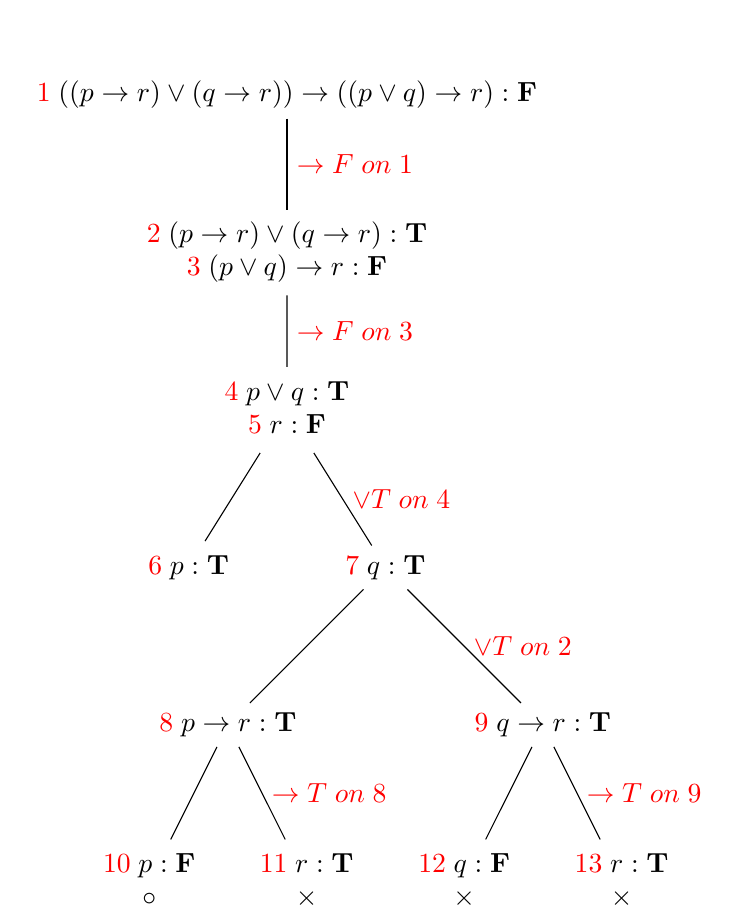
\begin{tikzpicture}

\node {$ \textcolor{red}{1}\; ((p \to r)\lor(q \to r))\to((p \lor q)\to r):\textbf{F} $} [sibling distance = 2.5cm] [level distance=20mm] 
        child {node {$ \begin{array}{c} \textcolor{red}{2}\; (p \to r)\lor(q \to r):\textbf{T} \\ \textcolor{red}{3}\; (p \lor q)\to r:\textbf{F} \end{array} $}  
            child {node {$ \begin{array}{c} \textcolor{red}{4}\; p \lor q:\textbf{T} \\ \textcolor{red}{5}\; r:\textbf{F} \end{array} $} 
                child {node {$ \begin{array}{c} \textcolor{red}{6}\; p:\textbf{T} \\ \end{array} $}}
                child {node {$ \textcolor{red}{7}\; q:\textbf{T} $} [sibling distance = 4cm]
                    child {node {$ \textcolor{red}{8}\; p \to r:\textbf{T} $} [sibling distance = 2cm]
                        child {node {$ \begin{array}{c} \textcolor{red}{10}\; p:\textbf{F} \\ \circ \end{array} $}}
                        child {node {$ \begin{array}{c} \textcolor{red}{11}\; r:\textbf{T} \\ \times \end{array} $}
                        edge from parent node [right, red] {$\to T\;on\; 8$}}} 
                    child {node {$ \textcolor{red}{9}\; q \to r:\textbf{T} $} [sibling distance = 2cm]
                        child {node {$ \begin{array}{c} \textcolor{red}{12}\; q:\textbf{F} \\ \times \end{array} $}}
                        child {node {$ \begin{array}{c} \textcolor{red}{13}\; r:\textbf{T} \\ \times \end{array} $ }
                        edge from parent node [right, red] {$\to T\;on\; 9$}}
                        edge from parent node [right, red] {$\lor T\;on\; 2$}}
                        edge from parent node [right, red] {$\lor T\;on\; 4$}}
                        edge from parent node [right, red] {$\to F\;on\; 3$}} 
                        edge from parent node [right, red] {$\to F\;on\; 1$}};

\end{tikzpicture}
\end{center}


The truth assignment that makes the formula false is:
\begin{itemize}
\item
p:\;\textbf{F}
\item
q:\;\textbf{T}
\item
r:\;\textbf{F}
\end{itemize}


\subsection{b)}

\begin{center}
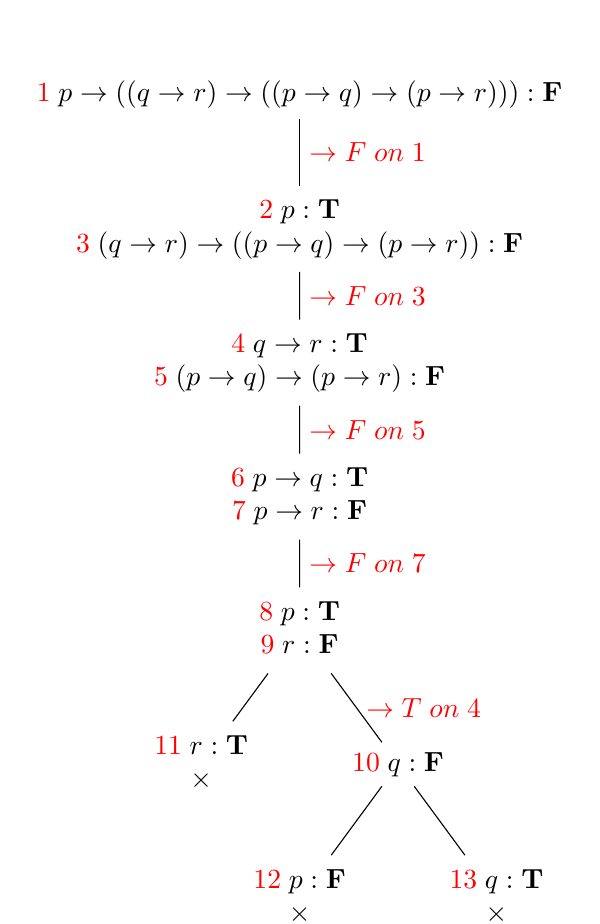
\begin{tikzpicture}

\node {$ \textcolor{red}{1}\; p \to ((q \to r)\to((p \to q)\to(p \to r))):\textbf{F} $} [sibling distance = 2.5cm] [level distance=17mm] 
        child {node {$ \begin{array}{c} \textcolor{red}{2}\; p:\textbf{T} \\ \textcolor{red}{3}\; (q \to r)\to((p \to q)\to(p \to r)):\textbf{F} \end{array} $} 
            child {node {$ \begin{array}{c} \textcolor{red}{4}\; q \to r:\textbf{T} \\ \textcolor{red}{5}\; (p \to q)\to(p \to r):\textbf{F} \end{array} $}
                child {node {$ \begin{array}{c} \textcolor{red}{6}\; p \to q:\textbf{T} \\ \textcolor{red}{7}\; p \to r:\textbf{F} \end{array} $}
                    child {node {$ \begin{array}{c} \textcolor{red}{8}\; p:\textbf{T} \\ \textcolor{red}{9}\; r:\textbf{F} \end{array} $}
                        child {node {$ \begin{array}{c} \textcolor{red}{11}\; r:\textbf{T} \\ \times \end{array} $}}
                        child {node {$ \textcolor{red}{10}\; q:\textbf{F} $}
                            child {node {$ \begin{array}{c} \textcolor{red}{12}\; p:\textbf{F} \\ \times \end{array} $}}
                            child {node {$ \begin{array}{c} \textcolor{red}{13}\; q:\textbf{T} \\ \times \end{array} $}}
                        edge from parent node [right, red] {$\to T\;on\; 4$}}
                        edge from parent node [right, red] {$\to F\;on\; 7$}}
                        edge from parent node [right, red] {$\to F\;on\; 5$}}
                        edge from parent node [right, red] {$\to F\;on\; 3$}} 
                        edge from parent node [right, red] {$\to F\;on\; 1$}};

\end{tikzpicture}
\end{center}

There is no truth assignment that makes the formula false, thus it is \underline{valid}.

 
\section{Exercise B}

From the inference, we can state the following state:

\begin{itemize}
\item
p: Per moves his bishop
\item
r: Ren\'e moves his rook 
\item
d: Per moves his queen
\item
b: Ren\'e breaks the chessboard
\end{itemize}

The inference becomes:

\begin{center}
$ p \to b $ \\
$ r \leftrightarrow d $ \\
$ \neg d \land \neg p $ \\
\noindent\rule{2.5cm}{0.4pt} \\
$ d \to (r \land b) $ \\
\end{center}

\newpage

Using the tableau method, we get the following:

\begin{center}
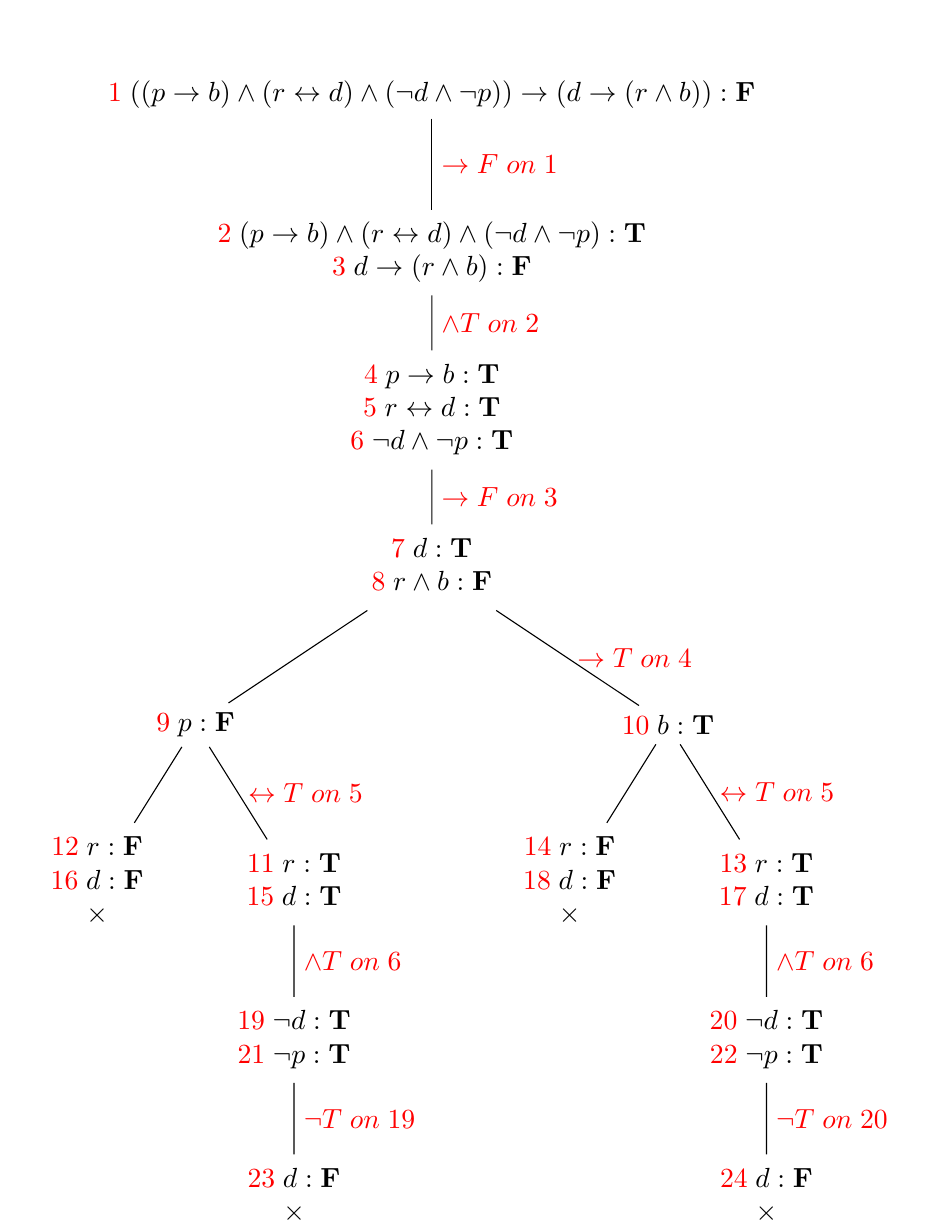
\begin{tikzpicture}

\node {$ \textcolor{red}{1}\; ((p \to b) \land (r \leftrightarrow d) \land (\neg d \land \neg p)) \to (d \to (r \land b)):\textbf{F} $} [sibling distance = 2cm] [level distance=20mm] 
        child {node {$ \begin{array}{c} \textcolor{red}{2}\; (p \to b) \land (r \leftrightarrow d) \land (\neg d \land \neg p):\textbf{T} \\ \textcolor{red}{3}\; d \to (r \land b):\textbf{F} \end{array} $} 
            child {node {$ \begin{array}{c} \textcolor{red}{4}\; p \to b:\textbf{T} \\ \textcolor{red}{5}\; r \leftrightarrow d:\textbf{T} \\ \textcolor{red}{6}\; \neg d \land \neg p:\textbf{T} \end{array} $}
                child {node {$ \begin{array}{c} \textcolor{red}{7}\; d:\textbf{T} \\ \textcolor{red}{8}\; r \land b:\textbf{F} \end{array} $} [sibling distance = 6cm]
                    child {node {$ \textcolor{red}{9}\; p:\textbf{F} $} [sibling distance = 2.5cm]
                        child {node {$ \begin{array}{c} \textcolor{red}{12}\; r:\textbf{F} \\ \textcolor{red}{16}\; d:\textbf{F} \\ \times \end{array} $}}
                        child {node {$ \begin{array}{c} \textcolor{red}{11}\; r:\textbf{T} \\ \textcolor{red}{15}\; d:\textbf{T}\end{array} $}
                        child {node {$ \begin{array}{c} \textcolor{red}{19}\; \neg d:\textbf{T} \\ \textcolor{red}{21}\; \neg p:\textbf{T}\end{array} $}
                        child {node {$ \begin{array}{c} \textcolor{red}{23}\; d:\textbf{F} \\ \times \end{array} $}
                        edge from parent node [right, red] {$\neg T\;on\; 19$}}
                        edge from parent node [right, red] {$\land T\;on\; 6$}}
                        edge from parent node [right, red] {$\leftrightarrow T\;on\; 5$}}}
                    child {node {$ \textcolor{red}{10}\; b:\textbf{T} $} [sibling distance = 2.5cm]
                        child {node {$ \begin{array}{c} \textcolor{red}{14}\; r:\textbf{F} \\ \textcolor{red}{18}\; d:\textbf{F} \\ \times \end{array} $}}
                        child {node {$ \begin{array}{c} \textcolor{red}{13}\; r:\textbf{T} \\ \textcolor{red}{17}\; d:\textbf{T}\end{array} $}
                        child {node {$ \begin{array}{c} \textcolor{red}{20}\; \neg d:\textbf{T} \\ \textcolor{red}{22}\; \neg p:\textbf{T}\end{array} $}
                        child {node {$ \begin{array}{c} \textcolor{red}{24}\; d:\textbf{F} \\ \times \end{array} $}
                        edge from parent node [right, red] {$\neg T\;on\; 20$}}
                        edge from parent node [right, red] {$\land T\;on\; 6$}}
                        edge from parent node [right, red] {$\leftrightarrow T\;on\; 5$}}
                        edge from parent node [right, red] {$\to T\;on\; 4$}}
                        edge from parent node [right, red] {$\to F\;on\; 3$}}
                        edge from parent node [right, red] {$\land T\;on\; 2$}} 
                        edge from parent node [right, red] {$\to F\;on\; 1$}};

\end{tikzpicture}
\end{center}

There is no truth assignment that makes the formula false, thus it is \underline{valid} and the inference is logically correct.
\section{Exercise C} 
\begin{enumerate}[label=\alph*)]

\item $ A= \{ x \in \mathbb{R} \; | \; x^2-3x=4 \} = \{ -1,4 \} $ \\
Please note that the above represents the equation $x^2-3x=4$ which can be solved with the quadratic formula. The solutions for the equations are $-1$ and $4$. The steps using the quadratic formula have not been shown.

\item $ B= \{ x \in \mathbb{Z} \; | \; -3 \le x < 3 \} = \{ -3,-2,-1,0,1,2 \} $

\item $ C= \{ x \in \mathbb{Z} \; | \; -3 \le x < 3 \land x^2-3x=4 \} = \{ -1 \} $ \\ 
Using set operation, we can write this as $ C= A \cap B $ because it represents all the common elements of set $A$ and $B$.

\item $ D= \{ x \in \mathbb{Z} \; | \; -3 \le x < 3 \land x^2-3x \ne 4 \} = \{ -3,-2,0,1,2 \} $ \\
Using set operation, we can write this as $ D = B - A $, because it represents all the elements that belong to $B$ and do not belong to $A$. Hence: \\ $ D= \{ x \in \mathbb{Z} \; | \; x \in B \land x \not\in A \} $.

\end{enumerate}

\section{Exercise D}
In order to show that the equalities hold we used propositional logic formulas and the truth table method.

\begin{enumerate}[label=\alph*)]

\item $ A \cup (B \cap C) = (A \cup B) \cap (A \cup C) $ \\
Translated into propositional logic becomes: \\ 
$ A \lor (B \land C) = (A \lor B) \land (A \lor C) $ \\
To which we can apply the distributive property of $\lor$ over $\land$ on the left hand side: \\
$ (A \lor B) \land (A \lor C) = (A \lor B) \land (A \lor C) $

\item $ A-(A \cap B) = A-B $ \\
Translated into propositional logic becomes: \\
$ A \land \neg(A \land B) = A \land \neg B $ \\
To which we can apply De Morgan's law on the left hand side: \\
$ A \land (\neg A \lor \neg B) = A \land \neg B $ \\
And then apply the distributive property of $\land$ over $\lor$ on the left hand side: \\
$ (A \land \neg A) \lor (A \land \neg B) = A \land \neg B $ \\
From here we can see that the block $(A \land \neg A)$ is always false, thus the following $\lor$ condition only depends on $A \land \neg B$. We can rewrite the equation in this form: \\
$ A \land \neg B = A \land \neg B $ 

\item $ A \cap (A \cup B) = A $  \\
Translated into propositional logic becomes: \\
$ A \land (A \lor B) = A $ \\
From here we can already say that the formula $A \land (A \lor B)$ is true only when $A$ is true. As a proof we construct the table from which we can see that $A \land (A \lor B)$ gets a true value only when $A$ is set to true.

\begin{center}
\begin{tabular}{ |c|c||c|c| } 
\hline
A & B & $A \lor B$ & $A \land (A \lor B)$  \\
\hline
\hline
T & T & T & T\\
\hline
T & F & T & T\\
\hline
F & T & T & F\\
\hline
F & F & F & F\\
\hline
\end{tabular}
\end{center}

 So the formula $A \land (A \lor B) = A$ is only dependent on A and can be rewritten as: \\
 $A=A$.
 
\end{enumerate}
\section{Exercise E}

\begin{enumerate}
\item 
Following the hint from the assignment text, we have the following propositional variables $s$ and $p$ which denotes: 
\begin{itemize}
    \item $p$ = "Peter is a truth sayer"
    \item $s$ = "Signe is a truth sayer"
\end{itemize}

From Peter, we know that at-least Peter or Signe is a liar. We can formulate the statement with: \\
$ \neg p \lor \neg s$ \\

To check whether Peter or Signe is the liar, we formulate a statement where Peter is set to be the truth sayer. This can be formulated with following statement:  \\
$p \leftrightarrow (\neg p \lor \neg s) $ \\

The following truth table can be constructed:
\begin{center}
\begin{tabular}{ |c|c||c|c|c|c| } 
\hline
$p$ & $s$ & $\neg p$ & $\neg s$ & $\neg p \lor \neg s$ & $p \leftrightarrow (\neg p \lor \neg s) $  \\
\hline
\hline
T & T & F & F & F & F\\
\hline
 \textcolor{red}{T} &  \textcolor{red}{F} & \textcolor{red}{F} & \textcolor{red}{T} & \textcolor{red}{T} &  \textcolor{red}{T}\\
\hline
F & T & T & F & T & F\\
\hline
F & F & T & T & T & F\\
\hline
\end{tabular}
\end{center}

Looking at the table, we can see which values of $p$ and $s$ make the formula true. In conclusion, we can see that Peter is telling the truth and Signe is lying. Hence, Peter is the truth sayer in this case.

\item
By using the hint from the assignment text, we can set the variables $a$ and $b$ to denote: 
\begin{itemize}
    \item $a$ = "Anne is a truth sayer"
    \item $b$ = "Bob is a truth sayer"
\end{itemize}

We can formulate the statement with: \\
$ \neg b \to \neg a$ \\

Again, we can check if Anne is telling the truth by formulating a statement where Anne is set to be the truth sayer. The statement can be formulated with: \\
$a \leftrightarrow (\neg b \to \neg a) $ \\

From the above equation, we have the following truth table:
\begin{center}
\begin{tabular}{ |c|c||c|c|c|c| } 
\hline
$a$ & $b$ & $\neg a$ & $\neg b$ & $\neg b \to \neg a$ & $a \leftrightarrow (\neg b \to \neg a) $  \\
\hline
\hline
\textcolor{red}{T} & \textcolor{red}{T} & \textcolor{red}{F} & \textcolor{red}{F} & \textcolor{red}{T} & \textcolor{red}{T}\\
\hline
T & F & F & T & F & F\\
\hline
F & T & T & F & T & F\\
\hline
F & F & T & T & T & F\\
\hline
\end{tabular}
\end{center}

Looking at the table, we can see which values of $a$ and $b$ make the formula true. In conclusion, we can see that Anne and Bob are both telling the truth. Since, if Bob is lying then Anne is also lying and vise versa. Therefore, both Anne and Bob are truth sayers. 


\item
From the assignment text, we have the following propositional variables:
\begin{itemize}
    \item $c$ = "Carsten is a truth sayer"
    \item $d$ = "Diana is a truth sayer"
    \item $e$ = "Erika is a truth sayer"
\end{itemize}

From Carsten, we have that only one of the three people are telling the truth. For that reason, we have the following: \\
$ ((c \land \neg d \land \neg e) \lor (\neg c \land d \land \neg e) \lor (\neg c \land \neg d \land e)) = claim$ \\

However, if Diana tells the truth, which is Carsten's claim regarding only one of them being a truth sayer, it must mean that the claim can only be true if Carsten is a truth sayer. Thereby, Carsten and Diana is a truth sayer if and only if Carsten's claim is true. This can be illustrated with the following equation: \\
$ d \to (c \to claim)$ \\

There's also the case where Diana is a truth sayer, but Carsten is not telling the truth. This means that there are two truth sayers because Carsten's claim about there only being one truth sayer is false. This can be illustrated with the following:\\
$ (d \land \neg c) \to e$ \\

Lastly, there is the case where Erika is telling the truth and Diana is lying. This can be illustrated like the following: \\
$e \leftrightarrow \neg d$ \\

Thus, we have the following combined equation: \\
$(d \to (c \to claim)) \land (d \land \neg c) \to e) \land (e \leftrightarrow \neg d)$ \\

From the above equation, a truth table can be constructed. In the truth table's last column is called all which represent the combined equation stated above:
\begin{center}
\begin{tabular}{ |c|c|c|c|c|c|c|c|c|c|c| } 
\hline
c & d & e & $\neg c$ & $\neg d$ & $\neg e$ & claim & $ d \to (c \to claim)$ & $e \leftrightarrow \neg d$ & $(d \land \neg c) \to e$ & All \\
\hline
\hline
F & T & T & T & F & F & F & T & F & T & F \\
\hline
\textcolor{red}{F} & \textcolor{red}{F} & \textcolor{red}{T} & \textcolor{red}{T} & \textcolor{red}{T} & \textcolor{red}{F} & \textcolor{red}{T} & \textcolor{red}{T} & \textcolor{red}{T} & \textcolor{red}{T} & \textcolor{red}{T} \\
\hline
T & T & T & F & F & F & F & F & F & T & F \\
\hline
T & T & F & F & F & T & F & F & T & T & F \\
\hline
T & F & F & F & T & T & T & T & F & T & F \\
\hline
\textcolor{red}{T} & \textcolor{red}{F} & \textcolor{red}{T} & \textcolor{red}{F} & \textcolor{red}{T} & \textcolor{red}{F} & \textcolor{red}{F} & \textcolor{red}{T} & \textcolor{red}{T} & \textcolor{red}{T} & \textcolor{red}{T} \\
\hline
F & T & F & T & F & T & T & T & T & F & F \\
\hline
F & F & F & T & T & T & F & T & F & T & F \\
\hline
\end{tabular}
\end{center}

It can be seen that are two cases. One where only Erika is a truth sayer, and one where both Erika and Carsten is telling the truth. However, we know know that Diana is lying. Hence, we cannot tell if Carsten is a truth sayer or not. Thus, Erika is the only truth sayer in this case. Therefore, the stranger should go with Erika. 

\end{enumerate}




\label{EndOfText}




\label{endOfDoc}
\end{document}
